\begin{frame}
    \frametitle{Introduction}

    \begin{itemize}
        \item The Tracker has been taking data since 2022 and has been doing it quite well.
        \item We see some potential issues in the 2026 data taking specifically in a specific module.
        \item This presentation will discuss this issue.
        \item We are quite early in understanding this.
        \item But thought it was best to make everyone aware of the situation.
        \item We will discuss the issue in a more “chronological” perspective rather than a diagnostic one.
    \end{itemize}

\end{frame}

\begin{frame}
    \frametitle{Quick Recap on Tracker}

    \begin{itemize}
        \item TODO: Add tracker diagram and explain the stations and layers.
        \item Explain numbering  of modules...
    \end{itemize}

\end{frame}

\begin{frame}
    \frametitle{First Observation\hfill \small{[Haruhi]}}

    \begin{itemize}
        \item First seen by Haruhi when trying to calculate unbaised residuals for 2026
        \item See \href{https://indico.cern.ch/event/1717284/}{Tracker Meeting Aug 12, 2026}.
    \end{itemize}

    \begin{figure}
        \begin{tikzpicture}
            \node[inner sep=0, outer sep=0] (img) at (0,0)
            {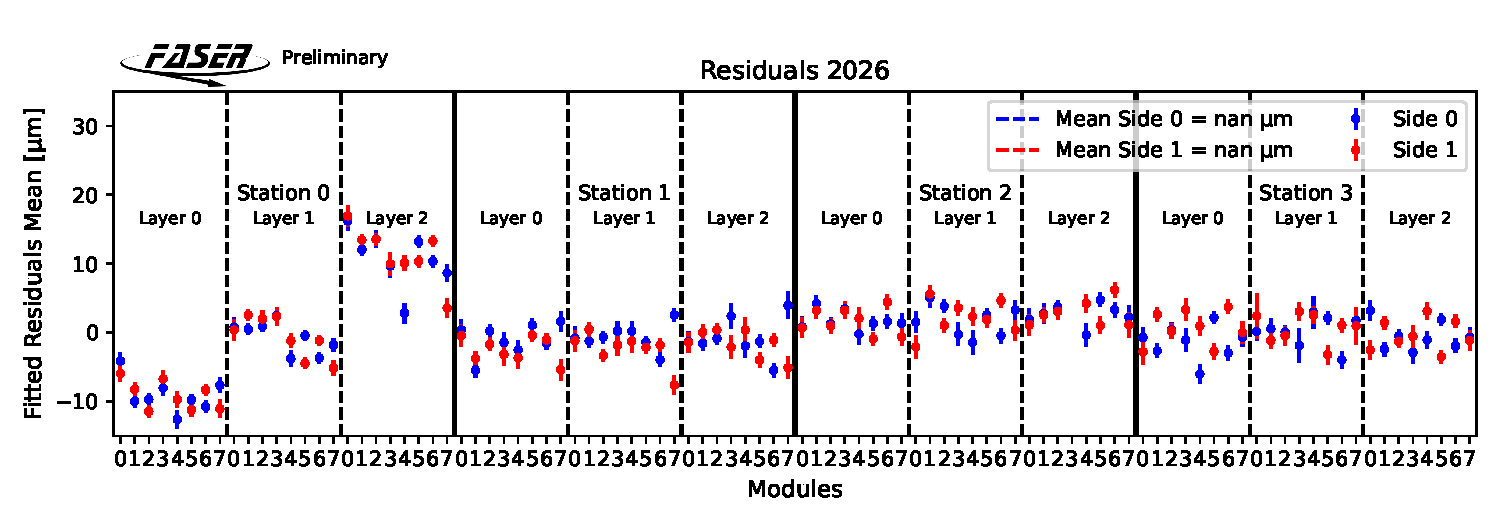
\includegraphics[width=\textwidth]{assets/Residual_Means_2026_4ST_forward.pdf}};

            \draw[red, thick]
            ($(img.south west)!0.71!(img.south east) + (0,0.1)$)
            rectangle
            node (rect) {}
            ($(img.south west)!0.72!(img.north east) + (0,0.7)$);

            \node[red, font=\footnotesize, anchor=north west] at ($(rect.south east)+(0.02,-1.5)$)
            {No entries in St2, L2, Mod.3};
        \end{tikzpicture}
    \end{figure}

\end{frame}

\begin{frame}
    \frametitle{Taking a closer look\hfill \small{[Haruhi]}}

    \begin{itemize}
        \item Initially suspected to be a fit failure/stats issue.
    \end{itemize}

    \begin{figure}
        \centering
        \begin{subfigure}{0.49\textwidth}
            \includegraphics[width=\textwidth, page=17]{assets/Residual_Distribution_4ST_2026_forward.pdf}
        \end{subfigure}
        \begin{subfigure}{0.49\textwidth}
            \includegraphics[width=\textwidth, page=18]{assets/Residual_Distribution_4ST_2026_forward.pdf}
        \end{subfigure}
    \end{figure}

    \begin{itemize}
        \item Quickly ruled out as nearby modules (in same station) had entries.
    \end{itemize}

\end{frame}

\begin{frame}
    \frametitle{Looking at Clusters/Space Points}
    \begin{figure}
        \centering
        \begin{subfigure}{0.49\textwidth}
            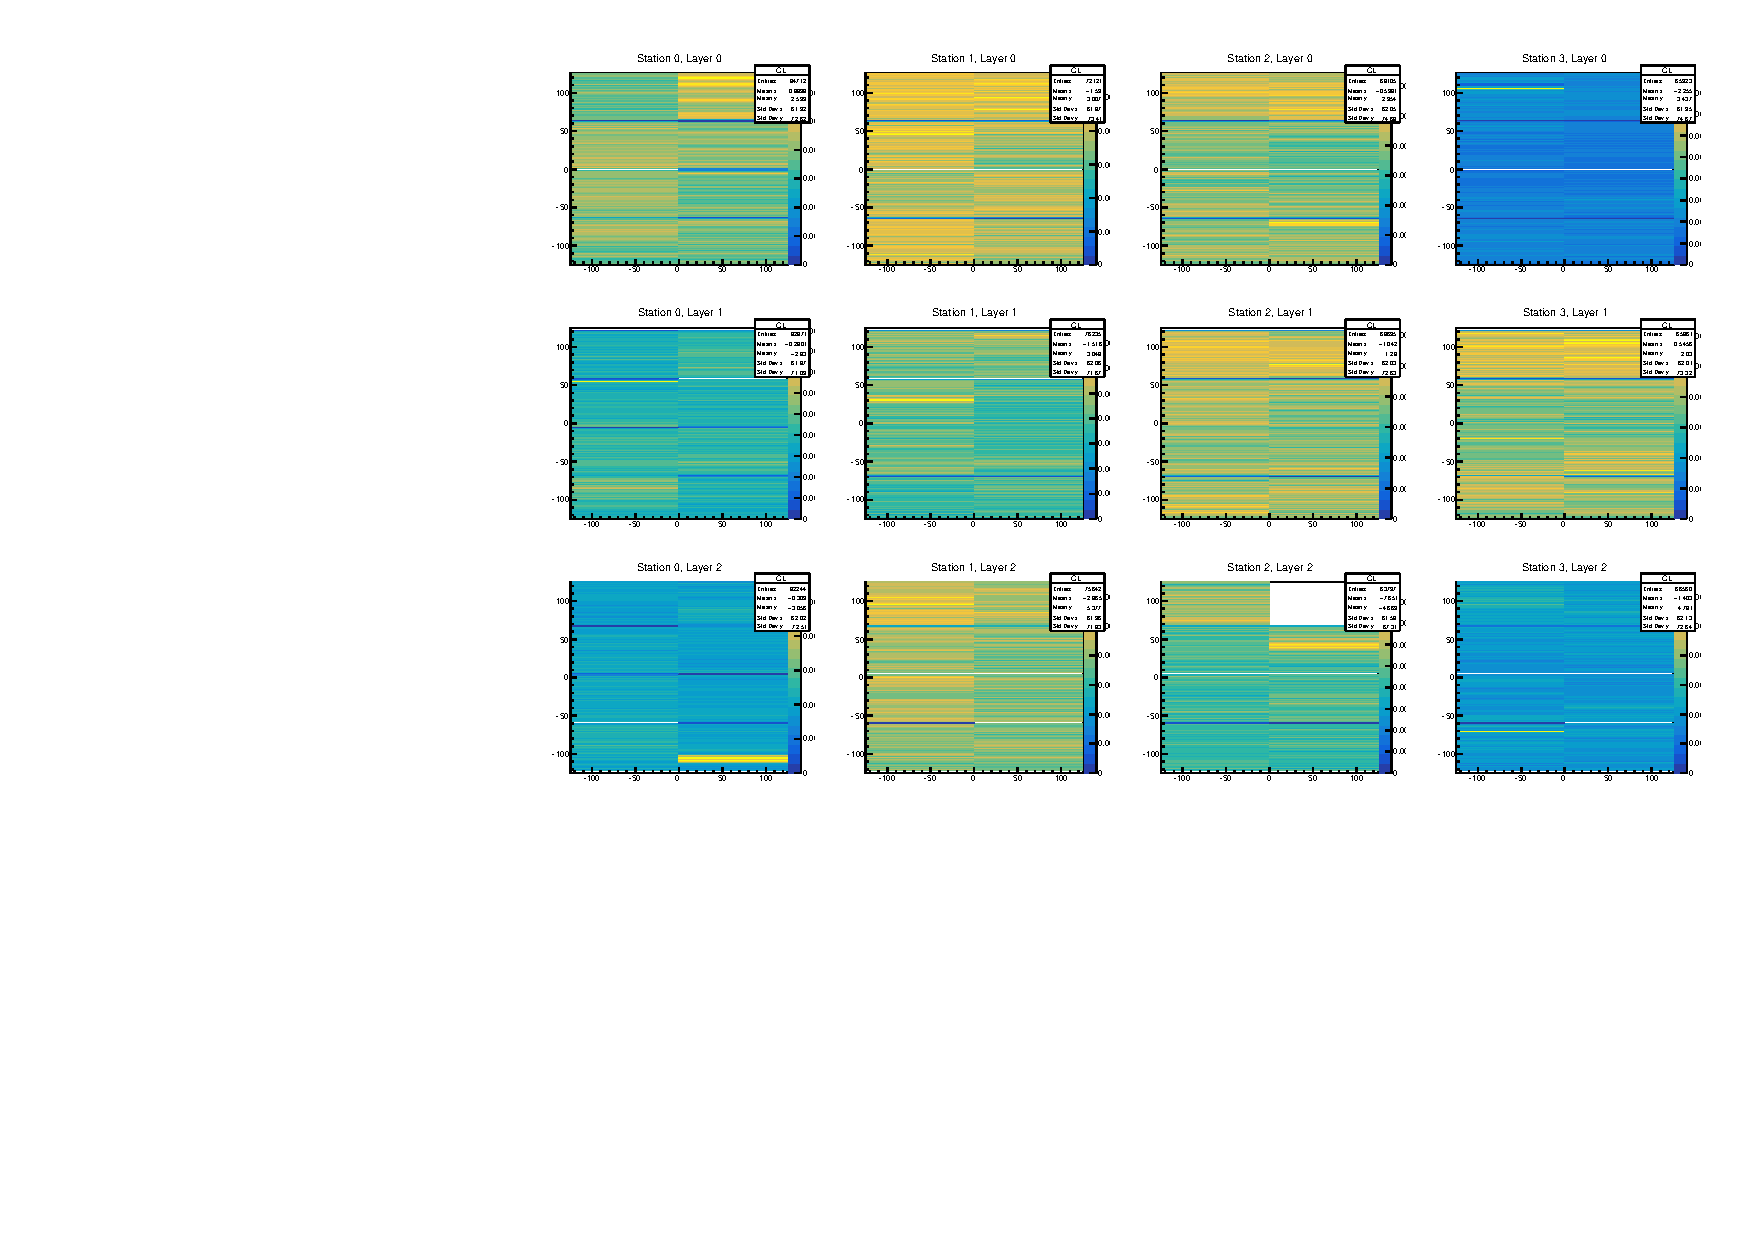
\includegraphics[width=\textwidth]{assets/Clusters_Nominal.pdf}
            \caption{Clusters from Run \#{022300}}
        \end{subfigure}
        \begin{subfigure}{0.49\textwidth}
            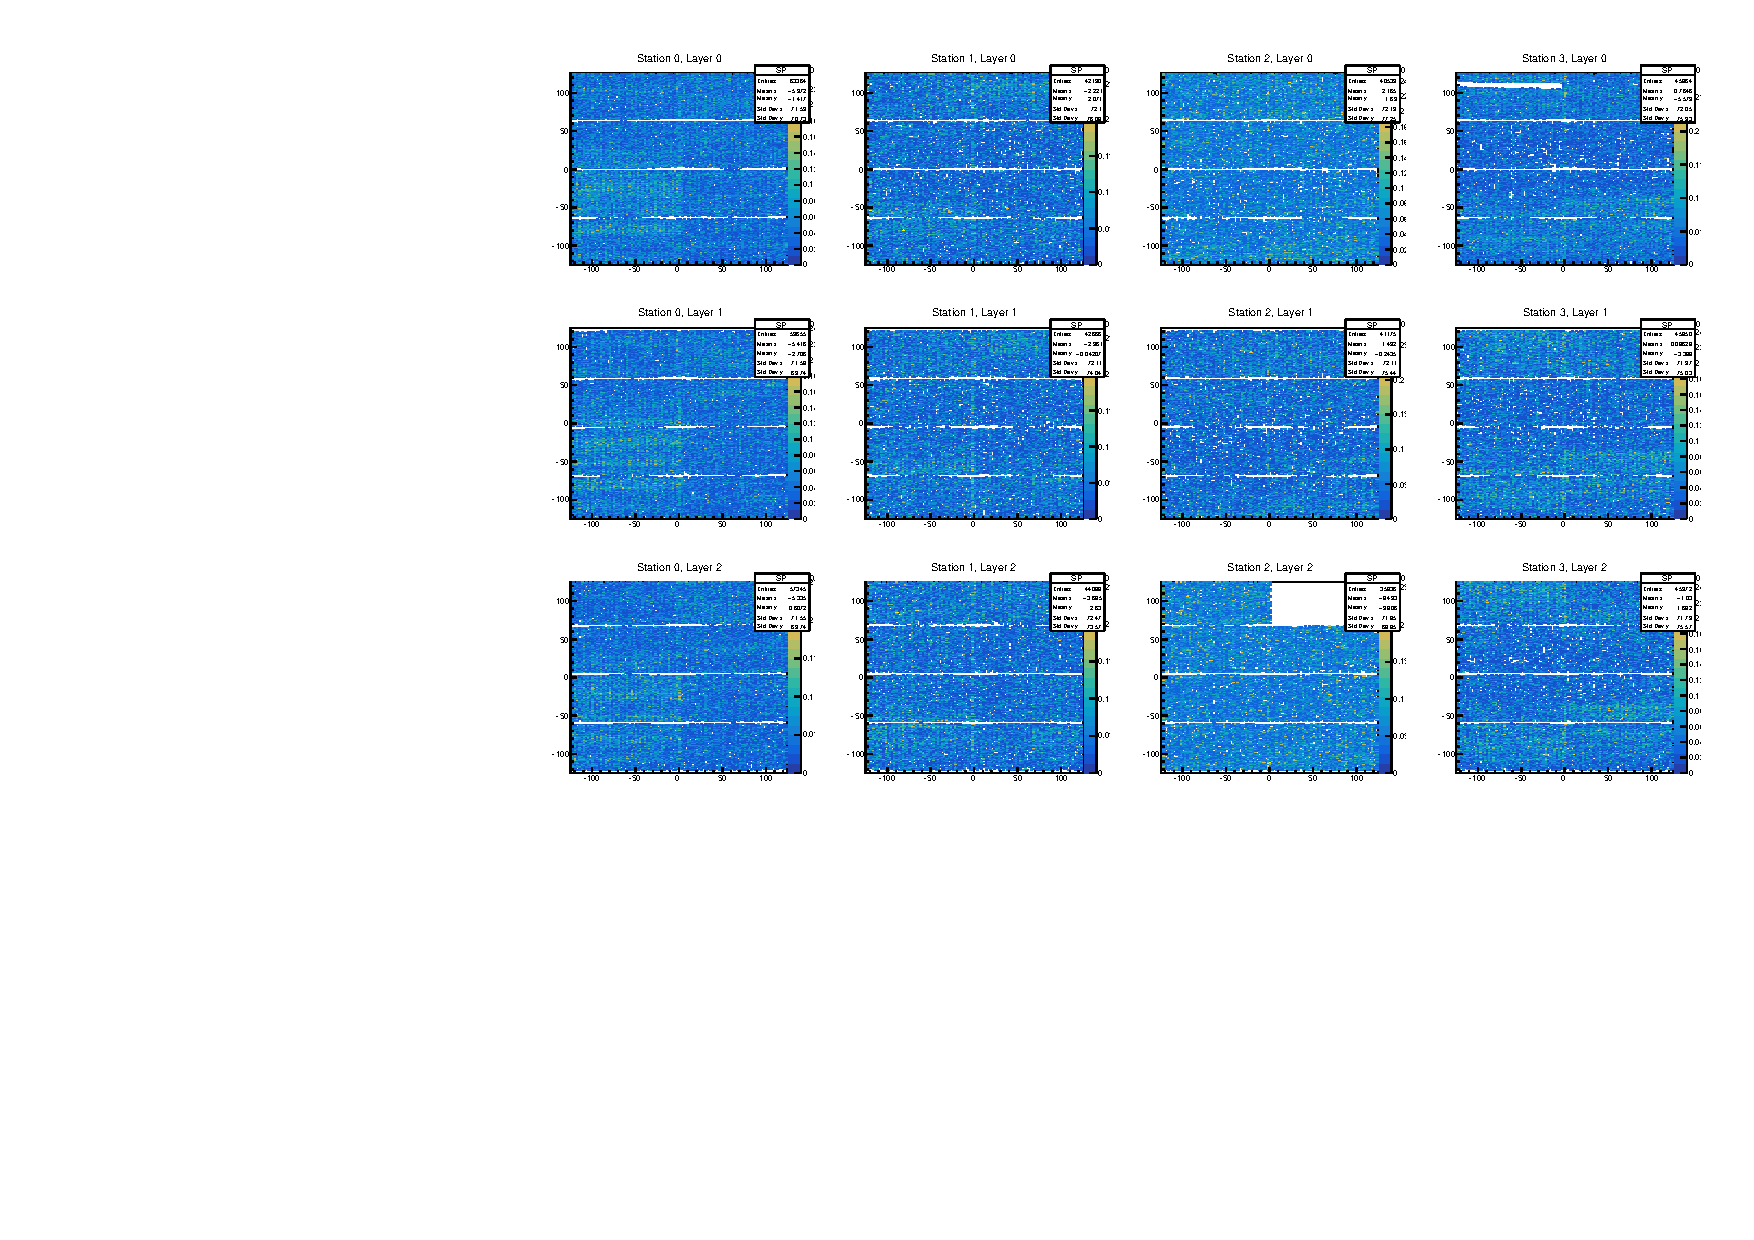
\includegraphics[width=\textwidth]{assets/SpacePoints_Nominal.pdf}
            \caption{Space Points from Run \#{022300}}
        \end{subfigure}
        \caption{SCT Clusters and Space Points from Run \#{022300}. Note that these are subset of the space points that are from the same layer.}
    \end{figure}
\end{frame}

\begin{frame}
    \frametitle{Similar Story with SCT Hits itself}
    \begin{figure}
        \centering
        % 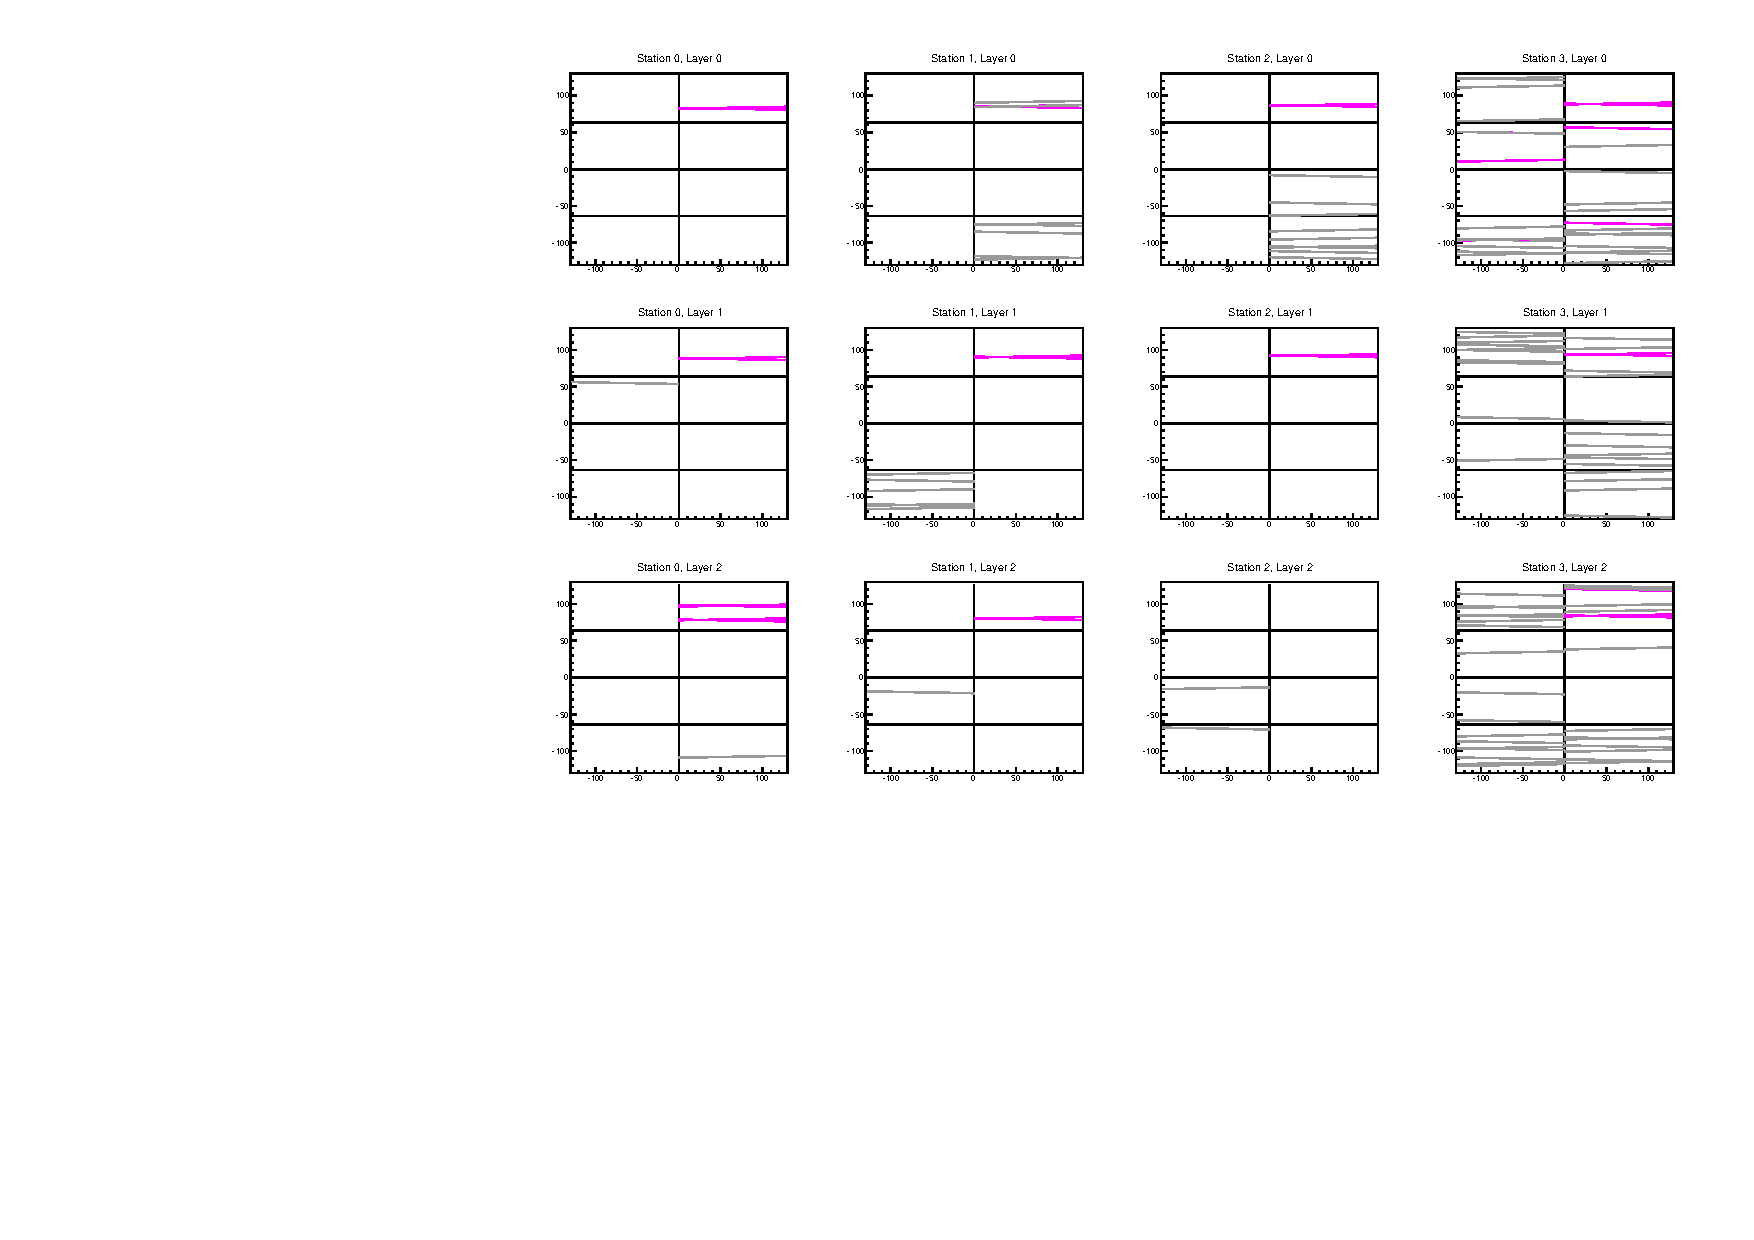
\includegraphics[height=0.75\textheight]{assets/SCTHits_Nominal.pdf}
        \begin{tikzpicture}
            \node[inner sep=0, outer sep=0] (img) at (0,0)
            {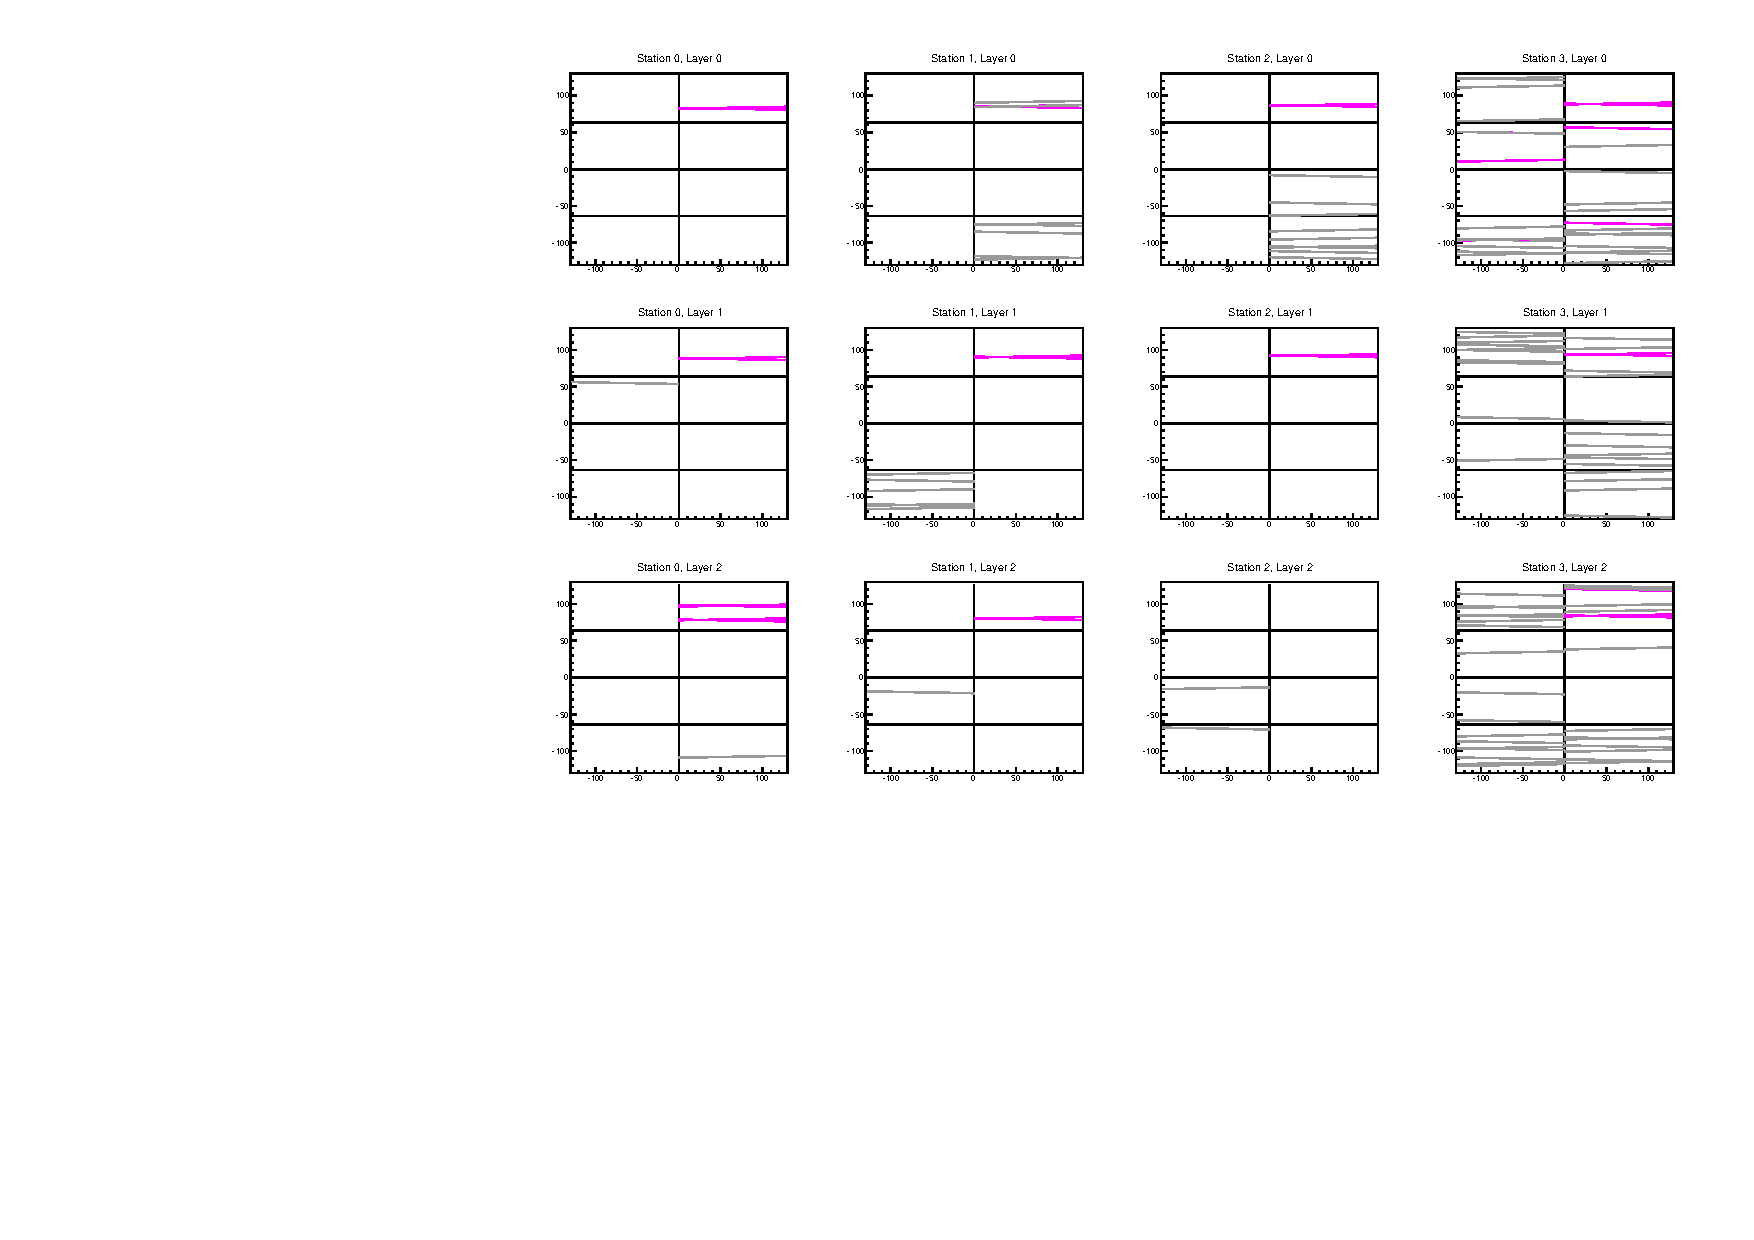
\includegraphics[width=0.70\textwidth]{assets/SCTHits_Nominal.pdf}};

            \draw[red, very thick]
            ($(img.south west)!0.625!(img.south east) + (0,1.85)$)
            rectangle
            node (rect) {}
            ($(img.south west)!0.715!(img.south east) + (0,1.45)$);
        \end{tikzpicture}
        \caption{SCT Hits from Event \#{2840829}, Run \#{022300}. Hits missing in the highlighted module.\\Note that out of time HITS (!\texttt{01X}) are shown in grey.}
    \end{figure}
\end{frame}

\begin{frame}
    \frametitle{What does the Track look like?}

    \begin{figure}
        \begin{tikzpicture}
            \node[inner sep=0, outer sep=0] (img) at (0,0)
            {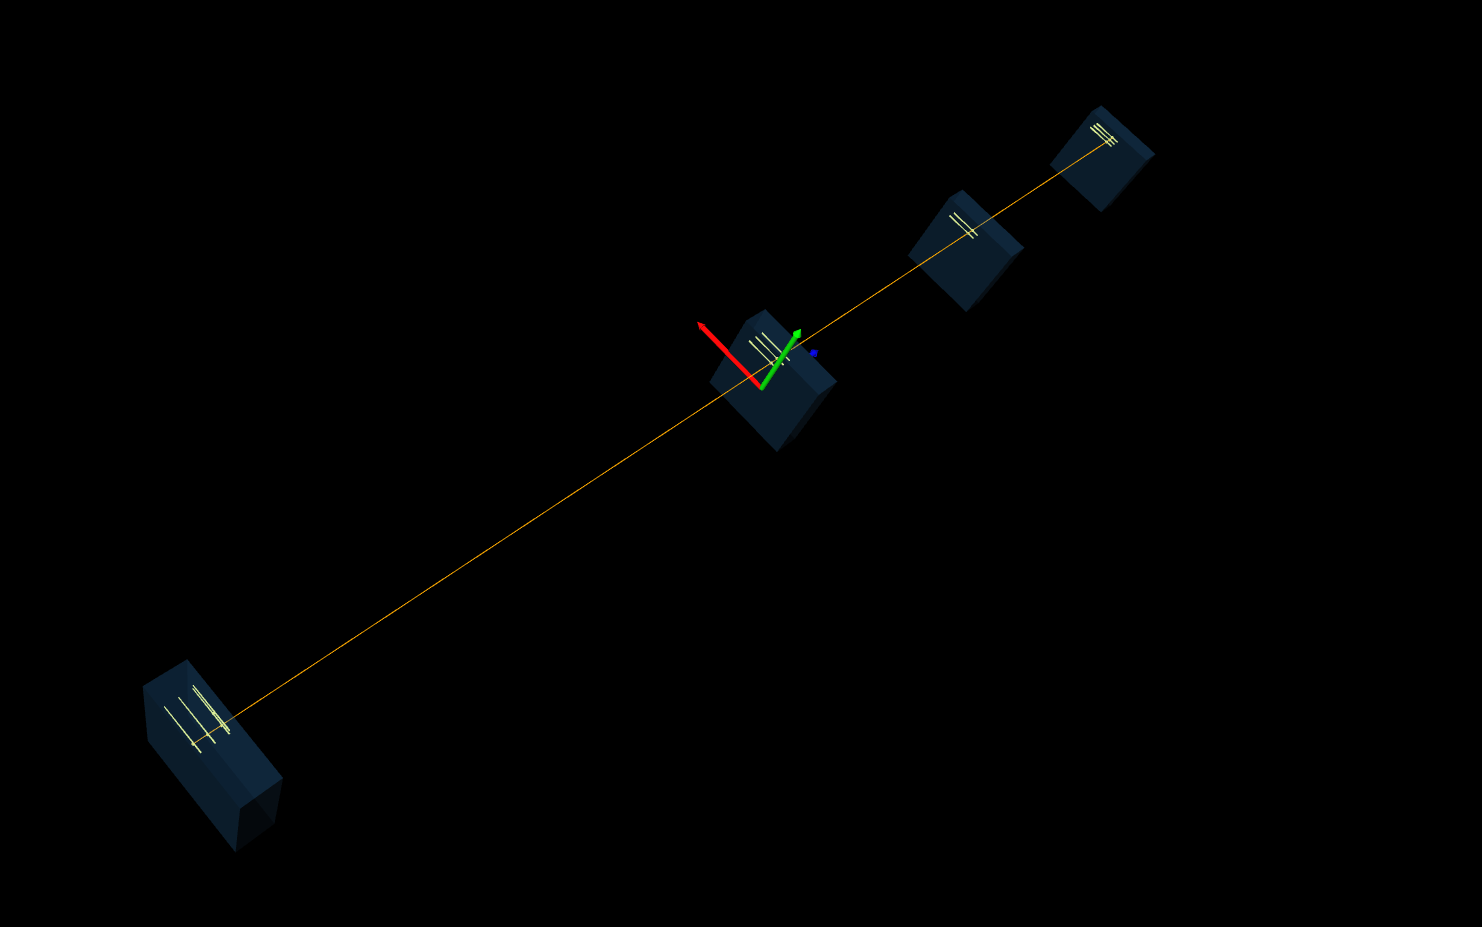
\includegraphics[width=0.7\textwidth]{assets/Event_Nominal.png}};

            \draw[red, thick]
            ($(img.north west)!0.65!(img.north east) + (-0.5,-1)$)
            rectangle
            node (rect) {}
            ($(img.north west)!0.68!(img.north east) + (0.2,-2.3)$);

            \node[red, font=\footnotesize, anchor=north west, align=center] at ($(rect.south east)+(0.02,-0.01)$)
            {Missing two clusters\\(St2, L2, Mod.3)};
        \end{tikzpicture}
        \caption{Event \#{2840829}, Run \#{022300}}
    \end{figure}

    % \begin{itemize}
    %     \item Note that in this case the track is still reconstructed.
    %     \item Although it now has two missing clusters, which is not ideal.
    % \end{itemize}

\end{frame}

\begin{frame}
    \frametitle{What \blueunderline{\it{could}} it mean for the Tracking?}

    \begin{itemize}
        \item It appears as though one module does not have any data
              \begin{itemize}
                  \item This is probably not completely true
              \end{itemize}
        \item In theory this should just be a reduction of two measurements in the final track
        \item \begin{itemize}
                  \item The Track-$\chi^2$ is lower for these events (\textcolor{red}{Add chi2 plots to backup})
                  \item But overall quality ($\chi^2$/NDF) is still good.
                  \item Impact on fiducial volume is around X\% (See slides from Oscar in backup)
              \end{itemize}
        \item More importantly, does the missing hits cause issues with track reconstruction?
              \begin{itemize}
                  \item This is a harder question to answer.
                  \item Needs a more detailed study to quantify this.
                  \item Ideally, shouldn't since the seeding should still pick up everything needed for the track.
              \end{itemize}
    \end{itemize}


\end{frame}

\begin{frame}
    \frametitle{Cluster Per Run}



\end{frame}

\begin{frame}
    \frametitle{Tracing out the timeline \hfill \small{[Oscar]}}

    \begin{figure}
        \centering
        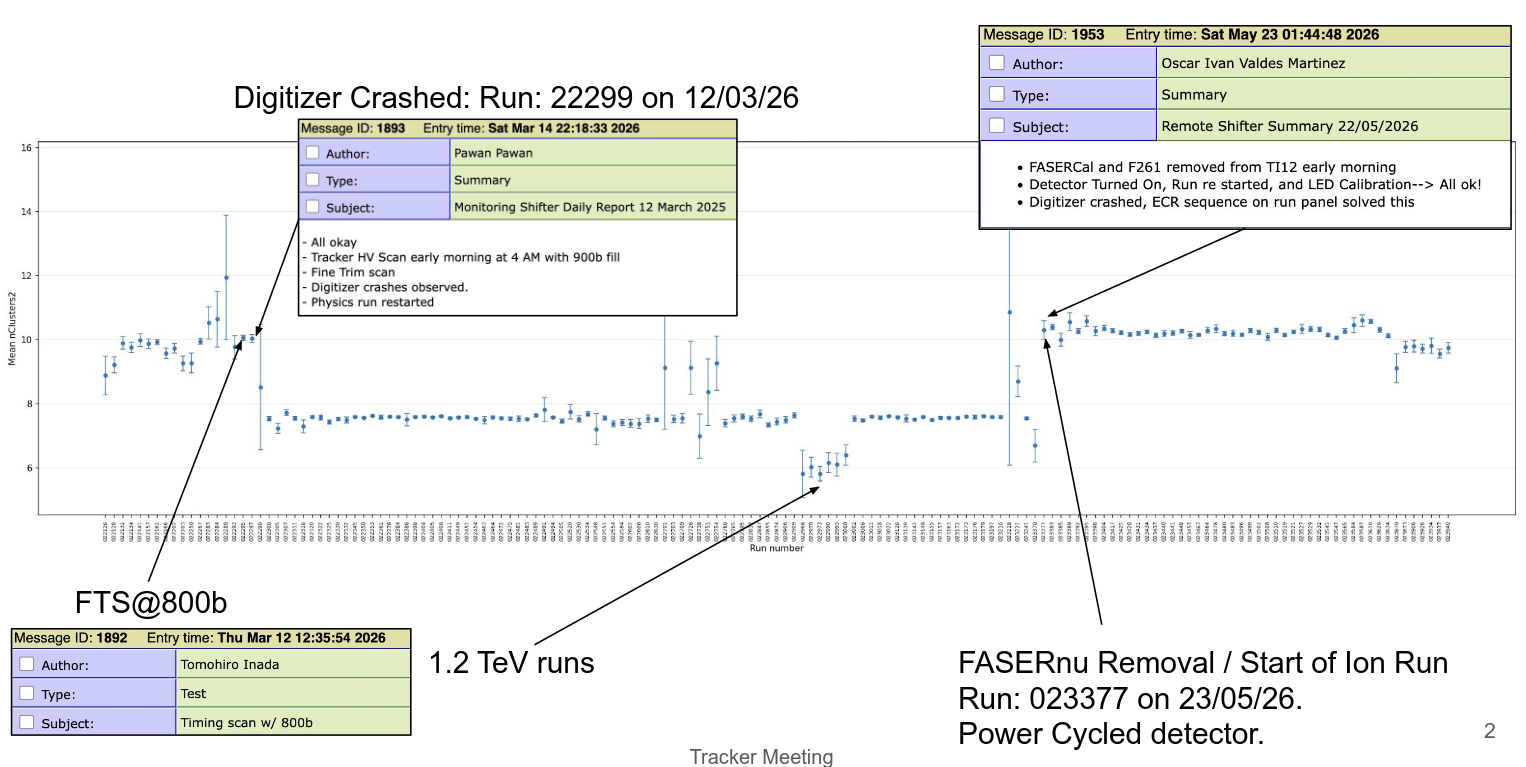
\includegraphics[width=0.9\textwidth]{assets/TimeLine_Oscar.png}
        \caption{Timeline of events from Oscar see {\href{https://indico.cern.ch/event/1721063/}{Tracker Meeting Aug 25 2026}}}
    \end{figure}
\end{frame}

\begin{frame}
    \frametitle{Timineline Summarized}

    \begin{itemize}
        \item Thursday Mar 12 2025: Fine Time Scan, after HV Scan
        \item Thursday Mar 12 2025: Fine time adjustment
        \item March 13-14 2025: Digitizer Crashes being observed
        \item
    \end{itemize}

\end{frame}

\begin{frame}
    \frametitle{Tangent: Possible Timing Issues?}



\end{frame}


\begin{frame}[fragile]
    \frametitle{Caveat: How do we read the raw data?}

    \begin{itemize}
        \item We saw that the SCT Raw Data was broken
        \item All of the checks so far uses \texttt{Calypso}
              \begin{itemize}
                  \item Brain pointed out that this implicitly assumes that \texttt{Calypso} decoded the data correctly.
              \end{itemize}
        \item This opens up new questions
              \begin{itemize}
                  \item Is the raw data actually broken? If so, why?
                  \item If not, why is \texttt{Calypso} not decoding it correctly?
                  \item Why isn't \texttt{Calypso} flagging an error?
              \end{itemize}
    \end{itemize}
\end{frame}

\begin{frame}[fragile]
    \frametitle{Reconstruction}

    \begin{itemize}
        \item Reconstruction does flag an error...But
    \end{itemize}
    \scriptsize{
        \begin{verbatim}
ToolSvc.TrackerDataDecoderTool            ERROR Online module 0 reports one or more errors.
        \end{verbatim}
    }
    \begin{itemize}
        % \item Note that the ``online'' module numbering is not the same as the ``offline'' one.
        \item This specific error is flagged from here \href{https://gitlab.cern.ch/faser/calypso/-/blob/master/Tracker/TrackerEventCnv/TrackerByteStream/src/TrackerDataDecoderTool.cxx#L174}{TrackerDataDecoderTool.cxx\#L174}
    \end{itemize}

    \scriptsize{
        \begin{verbatim}
          else if (sctEvent->HasError())
          {
            // FIXME: Should we return failure here?
            ATH_MSG_ERROR("Online module " << onlineModuleID << " reports one or more errors.");
            continue;
          }
        \end{verbatim}
    }

    \begin{itemize}
        \item While we report the error, we don't handle it in anyway, we ``continue'' over it.
        \item This is partly why we didn't catch it earlier in the prompt reconstruction.
              \begin{itemize}
                  \item this particular \blueunderline{module has an error flag} set in the raw data.
                  \item we \blueunderline{don't consider this a failure} and we \blueunderline{don't load the data} for the module.
                  \item other modules in the same event are still loaded and processed.
                  \item and we still \blueunderline{continue the reconstruction albeit with ``missing'' data}.
              \end{itemize}
    \end{itemize}


\end{frame}

\begin{frame}
    \frametitle{End Result}

    \begin{itemize}
        \item We have a valid ``event'' once \texttt{Calypso} is done reading the raw data.
              \begin{itemize}
                  \item This event does not really have any data from the specific module.
                  \item If the track did not pass through the module, then it is not a problem.
                  \item But if it did, then we don't use the specific SCT HITs.
              \end{itemize}
    \end{itemize}

    \begin{itemize}
        \item Only way to stumble on this would be
              \begin{itemize}
                  \item Either by looking for ERRORs in the log
                        \begin{itemize}
                            \item Note that this isn't guaranteed due to messaging limits \href{https://gitlab.cern.ch/atlas/Gaudi/-/blob/master/GaudiCoreSvc/src/MessageSvc/MessageSvc.cpp\#L333}{(see \texttt{MessageSvc.cpp\#L333})}
                            \item Do need to check if this is the case here.
                        \end{itemize}
                  \item Or by specifically looking for the tracks that pass through this module
                        \begin{itemize}
                            \item this we do not usually do
                            \item we briefly did this for 2024 data (see \href{https://gitlab.cern.ch/papawan/Presentations/-/raw/main/DQFollowUp\_PPT\_detailed/build/TrackDQ\_2024\_Deltailed\_Pawan.pdf}{Track DQ 2024})
                        \end{itemize}
              \end{itemize}
        \item Ideally if we have an error we should stop and handle it
    \end{itemize}

\end{frame}

\begin{frame}[fragile]
    \frametitle{So... Whats wrong with the raw data?\hfill \small{[Brain]}}

    \begin{itemize}
        \item The raw data dump has no errors nominally
              \begin{itemize}
                  \item Unless you run in debug mode
              \end{itemize}
    \end{itemize}
    \scriptsize{
        \begin{verbatim}
[ERROR] (file = TrackerDataFragment.icc)(func = DecodeModuleData)(line = 271) 
        | TrackerDataFragment::DecodeModuleData :: Module Data: ERROR code 0x1 for chip 9
        \end{verbatim}
    }

    \begin{itemize}
        \item This is the decoding error that was flagged in the reconstruction.
        \item Still investigating as to what is the exact cause of this error.
    \end{itemize}

    \begin{figure}
        \centering
        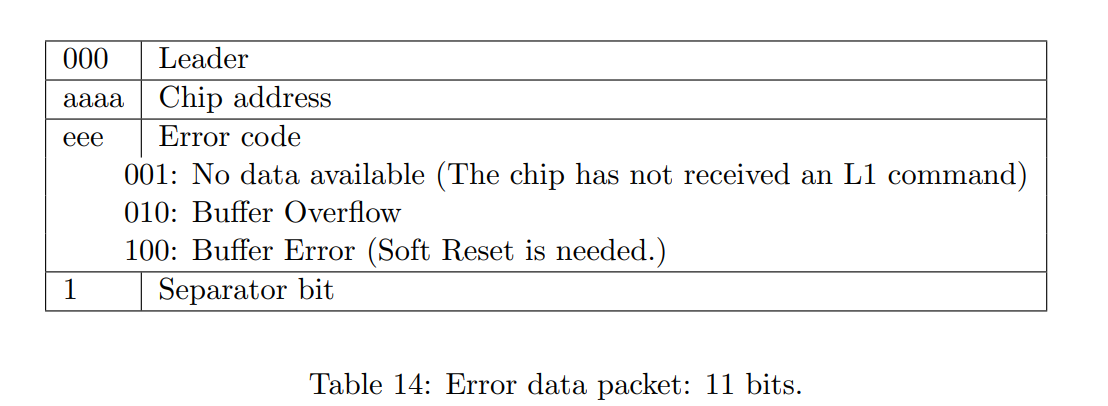
\includegraphics[width=0.5\textwidth]{assets/ErrorCode.png}
        \caption{\href{https://cern.sharepoint.com/sites/faser-share/Shared\%20Documents/Forms/AllItems.aspx?id=\%2Fsites\%2Ffaser-share\%2FShared\%20Documents\%2FTracker\%2FTracker\%20readout\%20board\%2FFASER\%20TRB\%20specification\%20v1.0.1.pdf\&parent=\%2Fsites\%2Ffaser-share\%2FShared\%20Documents\%2FTracker\%2FTracker\%20readout\%20board&p=true&ga=1}{Tracker Readout Spec}}
    \end{figure}

\end{frame}

\begin{frame}[fragile]
    \frametitle{Is it recoverable?}

    \begin{itemize}
        \item It is still unclear.
        \item A preliminary test was to comment out this error check in \texttt{Calypso}.
    \end{itemize}


    \scriptsize{
        \begin{verbatim}
          else if (sctEvent->HasError())
          {
            // FIXME: Should we return failure here?
            ATH_MSG_ERROR("Online module " << onlineModuleID << " reports one or more errors.");
            // continue;
            //Let's fill the data and see what happens
          }
        \end{verbatim}
    }

    \begin{itemize}
        \item This seems to run \textcolor{red}{none of the other checks are triggered (? Pawan: Verify this)}
              \begin{itemize}
                  \item This is probably a good sign.
              \end{itemize}
        \item This is not a proper fix, but just a test to see if data is recovered.
              \begin{itemize}
                  \item Still need to identify and fix the root cause of the error.
                  \item If not fixable, then we need to handle it correctly in the reconstruction.
              \end{itemize}
        \item Some results in the next slides.
    \end{itemize}

\end{frame}

\begin{frame}
    \frametitle{Cluster and Space Points after disabling the check}
    \begin{figure}
        \centering
        \begin{subfigure}{0.49\textwidth}
            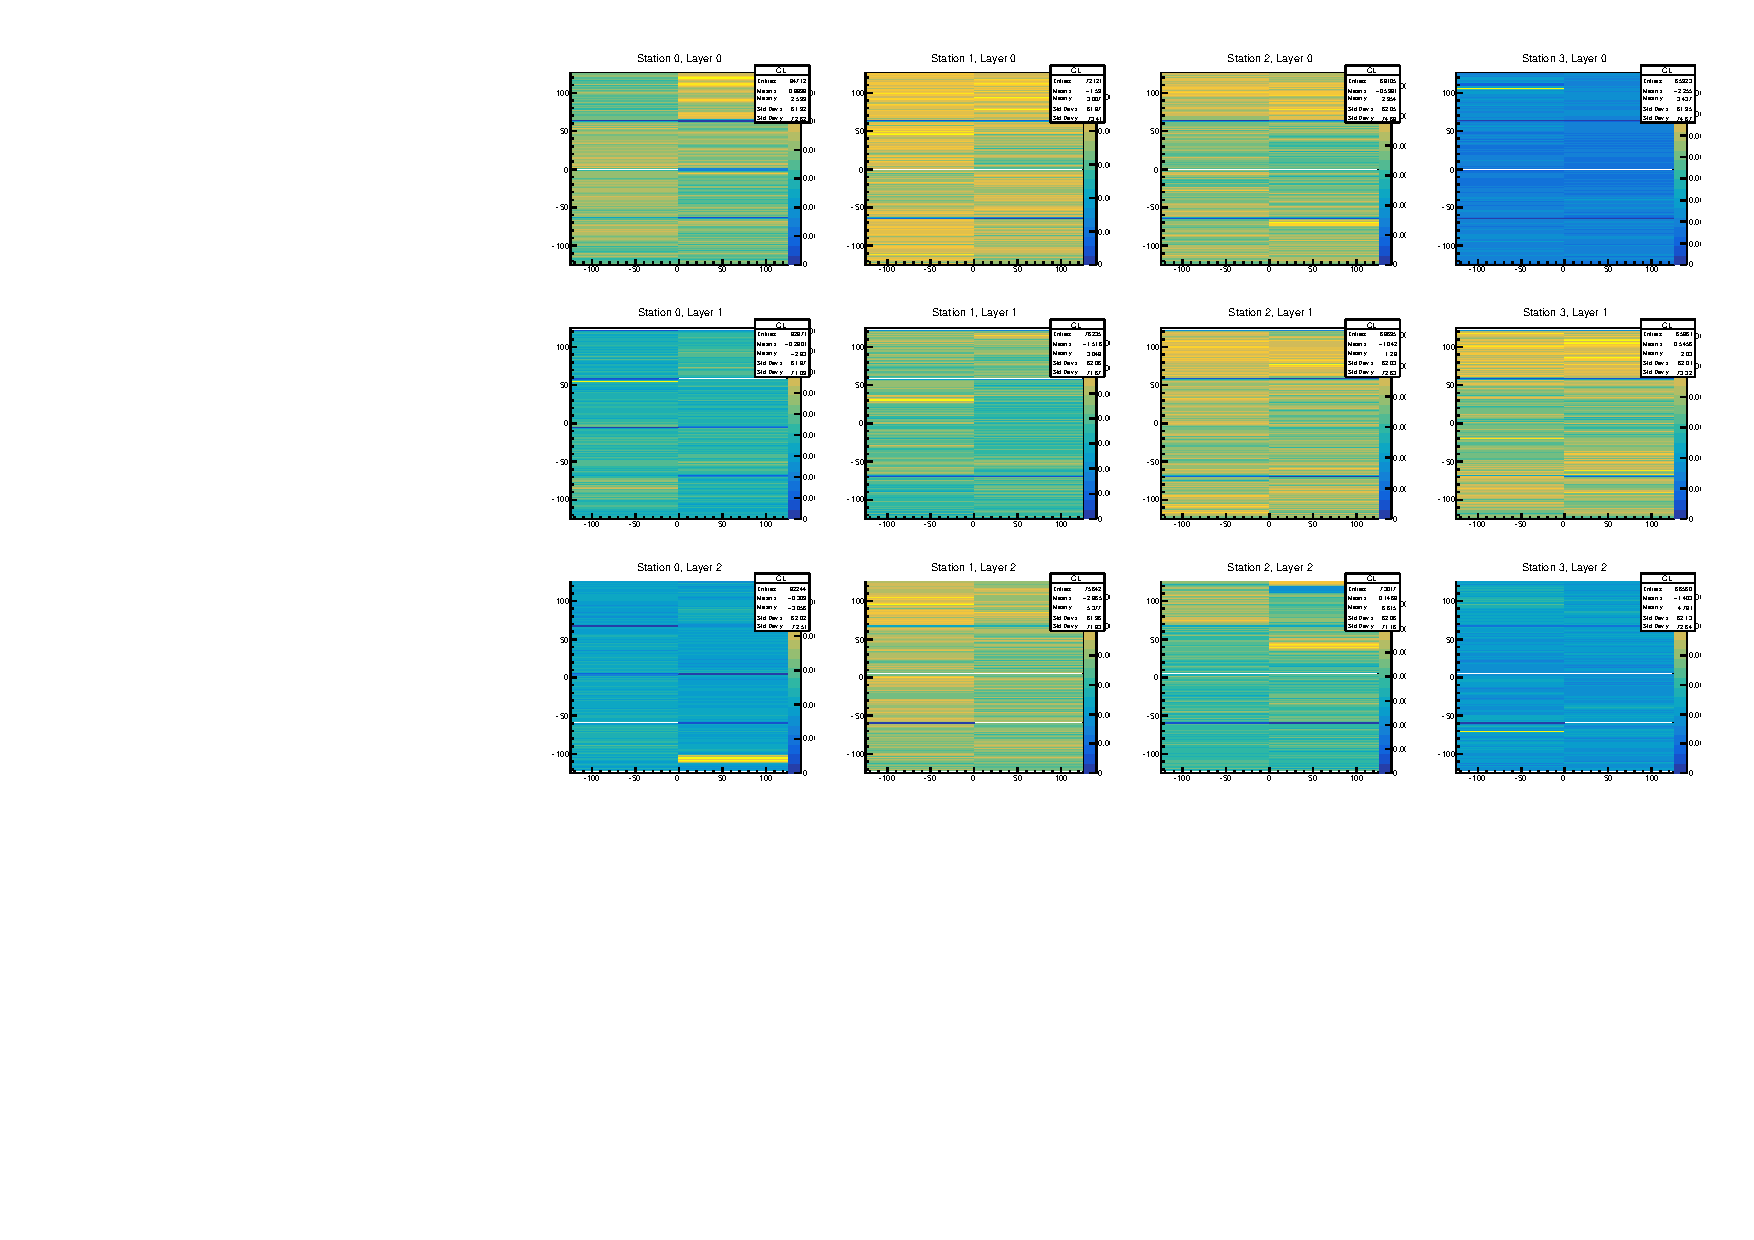
\includegraphics[width=\textwidth]{assets/Clusters_Patched.pdf}
            \caption{Clusters from Run \#{022300}}
        \end{subfigure}
        \begin{subfigure}{0.49\textwidth}
            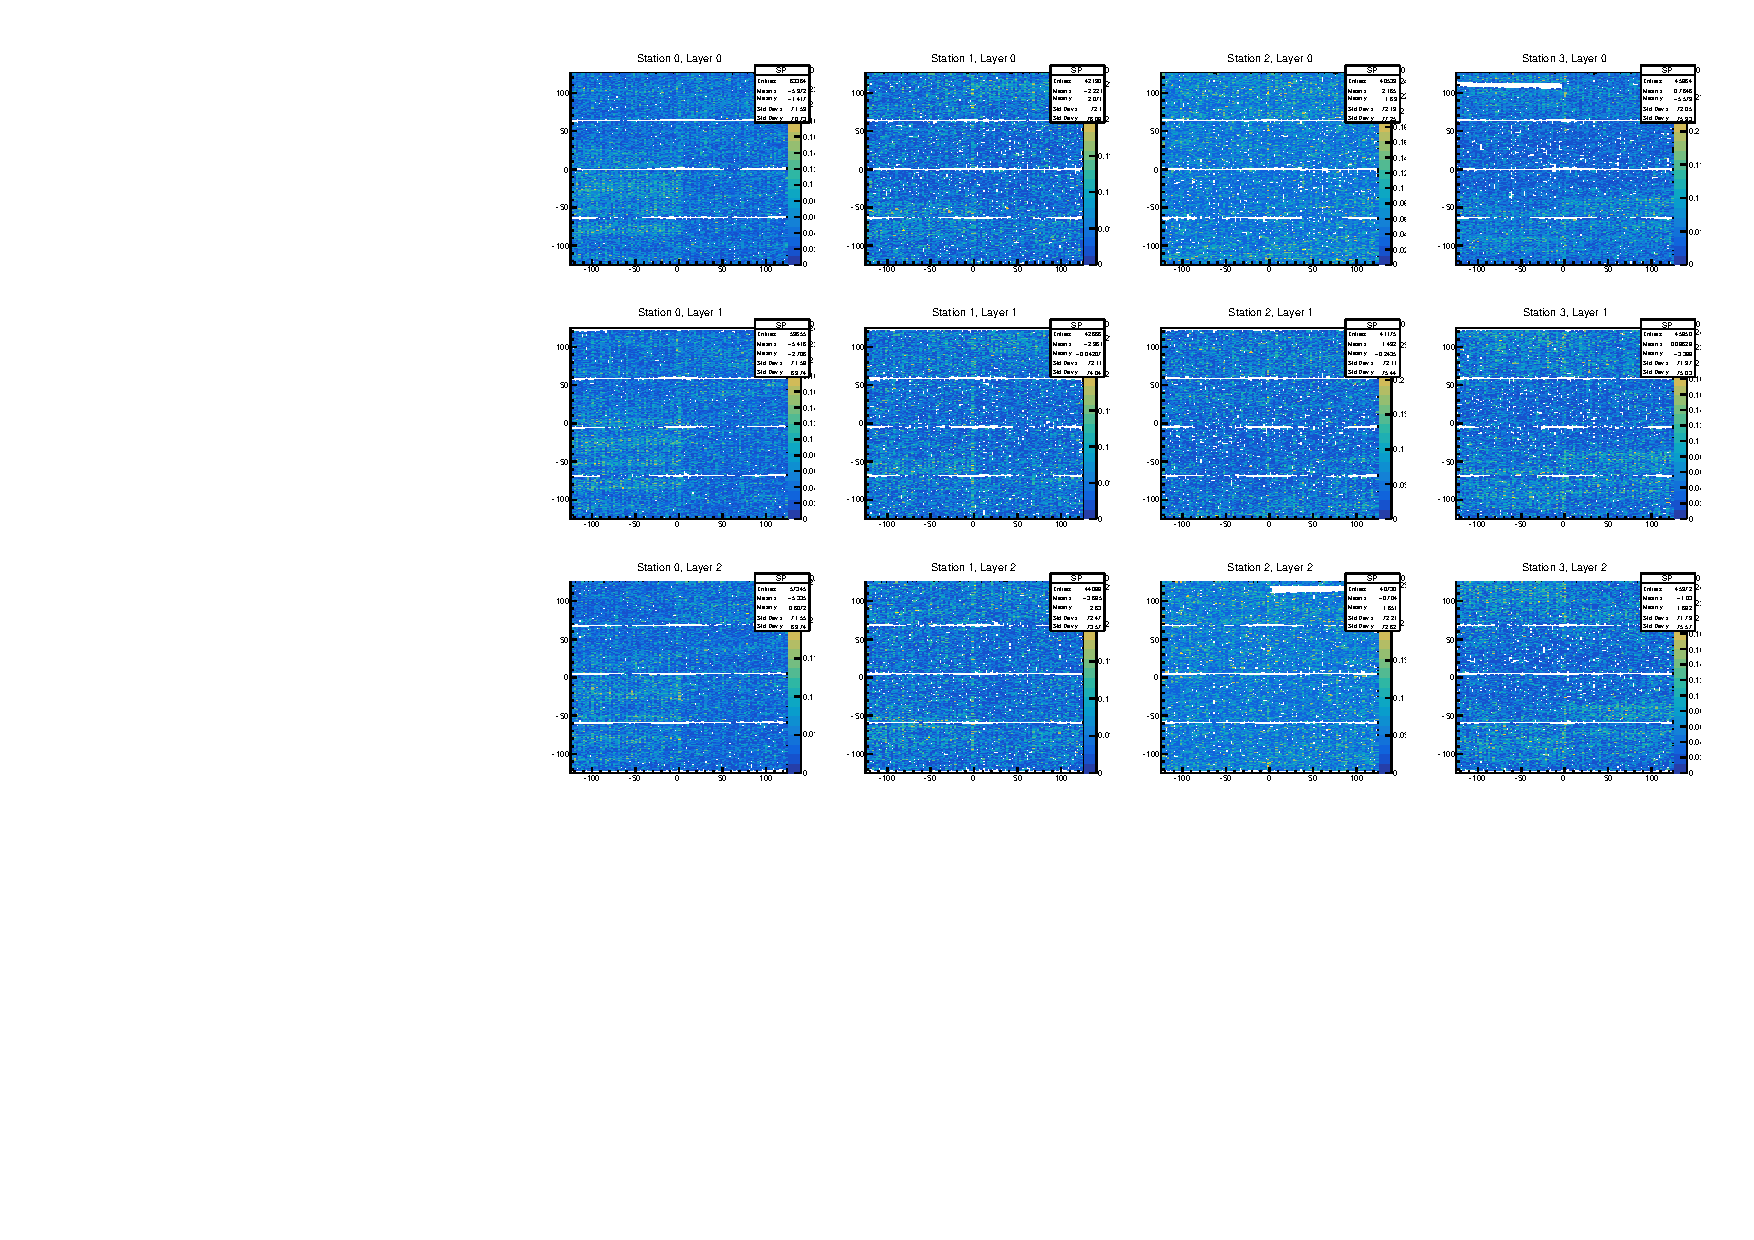
\includegraphics[width=\textwidth]{assets/SpacePoints_Patched.pdf}
            \caption{Space Points from Run \#{022300}}
        \end{subfigure}
        \caption{SCT Clusters and Space Points from Run \#{022300} after disabling the error check mentioned above.}
    \end{figure}

\end{frame}

\begin{frame}
    \frametitle{SCT Hits}
    \begin{figure}
        \centering
        % 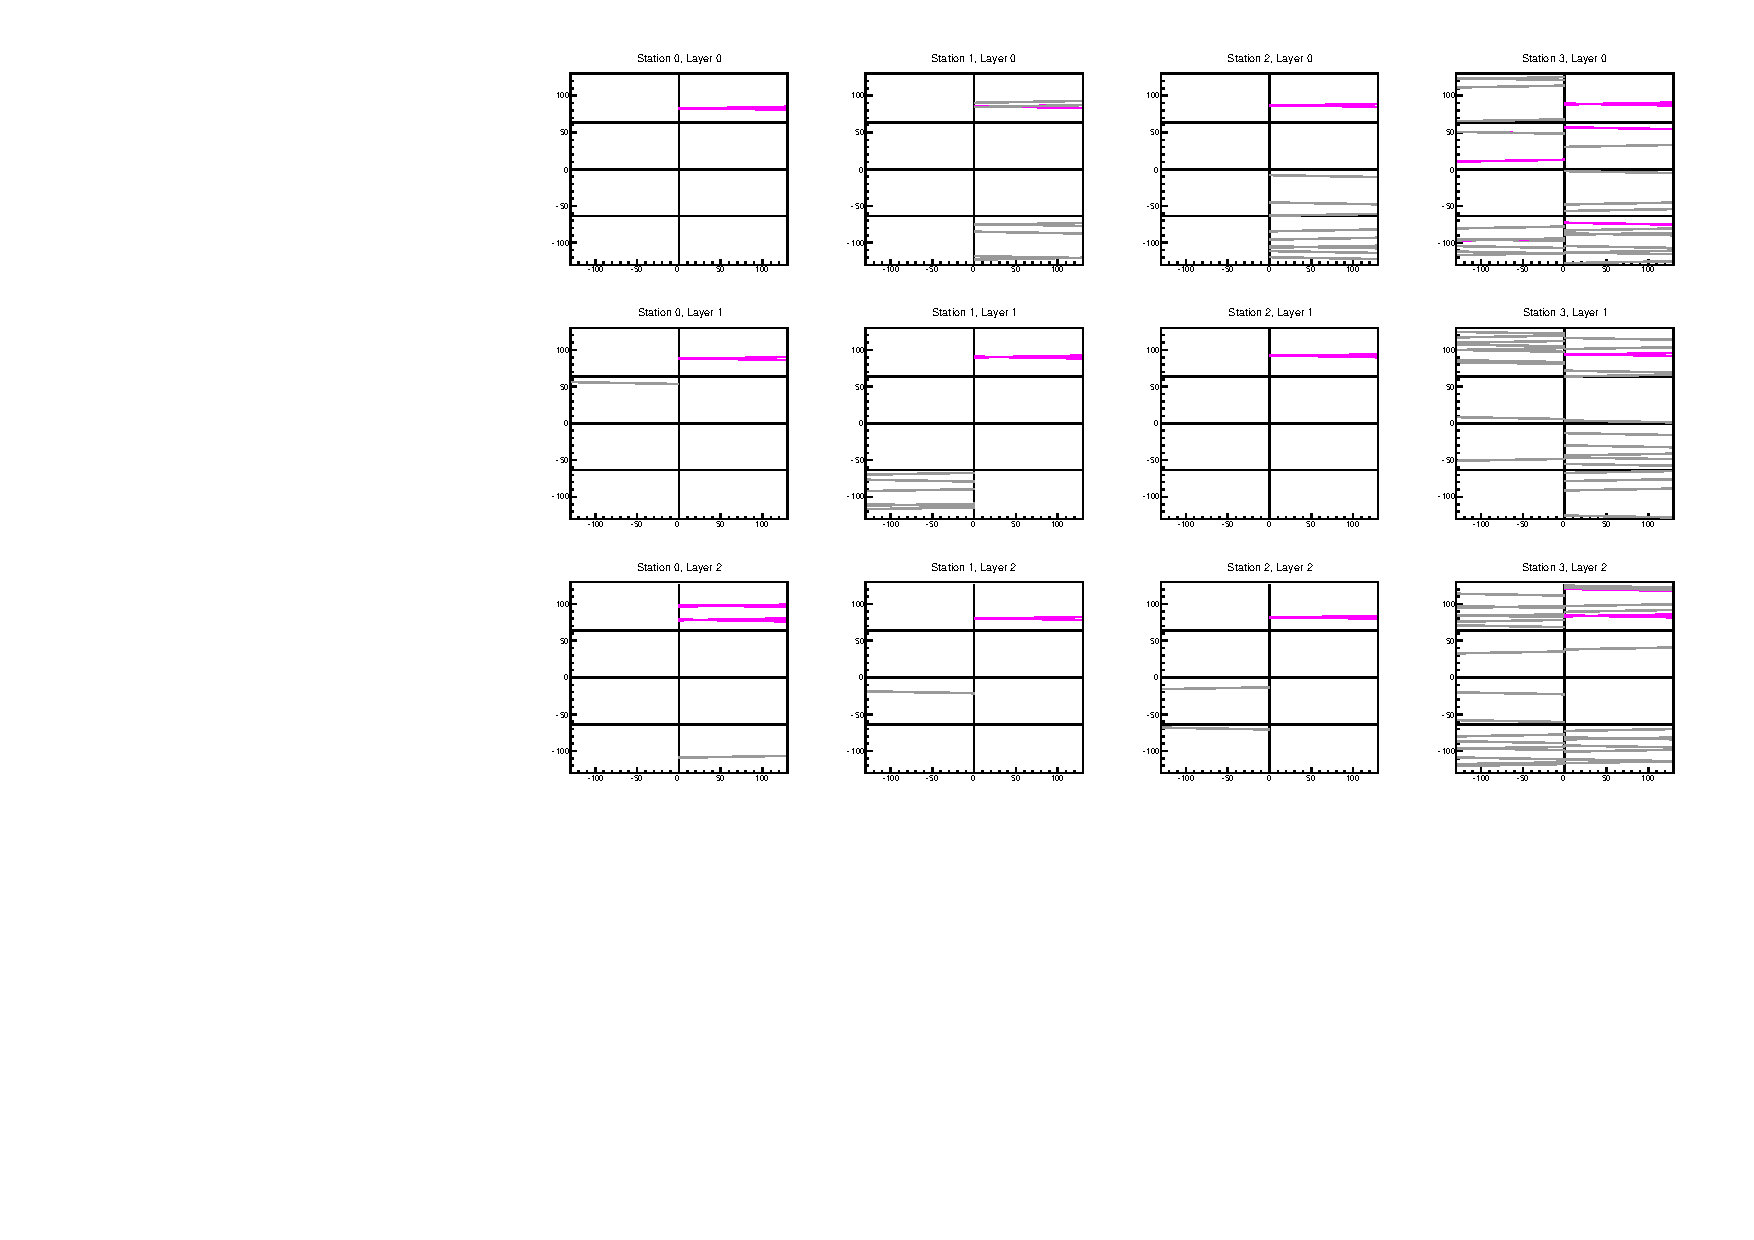
\includegraphics[height=0.75\textheight]{assets/SCTHits_Patched.pdf}
        \begin{tikzpicture}
            \node[inner sep=0, outer sep=0] (img) at (0,0)
            {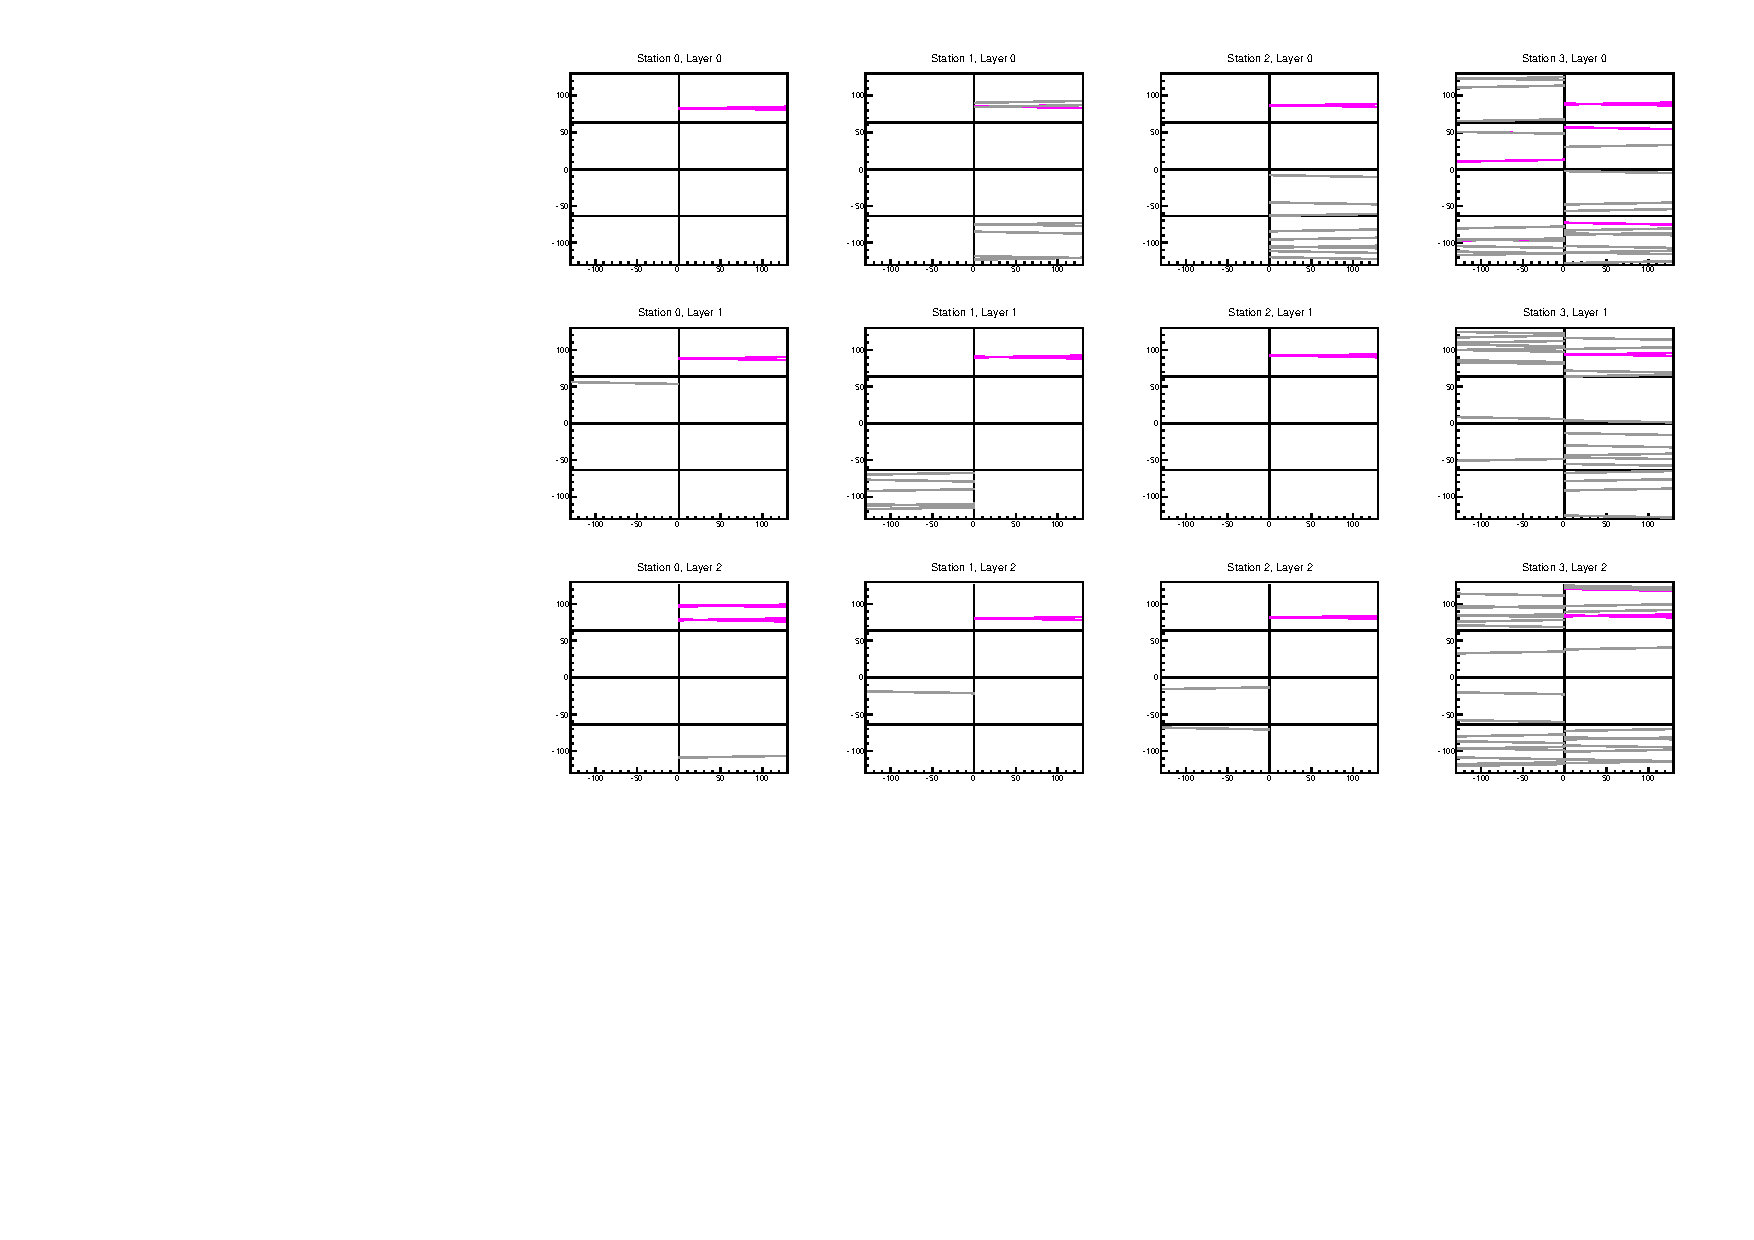
\includegraphics[width=0.70\textwidth]{assets/SCTHits_Patched.pdf}};

            \draw[red, very thick]
            ($(img.south west)!0.625!(img.south east) + (0,1.85)$)
            rectangle
            node (rect) {}
            ($(img.south west)!0.715!(img.south east) + (0,1.45)$);
        \end{tikzpicture}
        \caption{SCT Hits from Event \#{2840829}, Run \#{022300} after disabling the error check mentioned above.Hits are restored(?) in the highlighted module.}
    \end{figure}
\end{frame}

\begin{frame}
    \frametitle{Final Track}

    \begin{figure}
        \begin{tikzpicture}
            \node[inner sep=0, outer sep=0] (img) at (0,0)
            {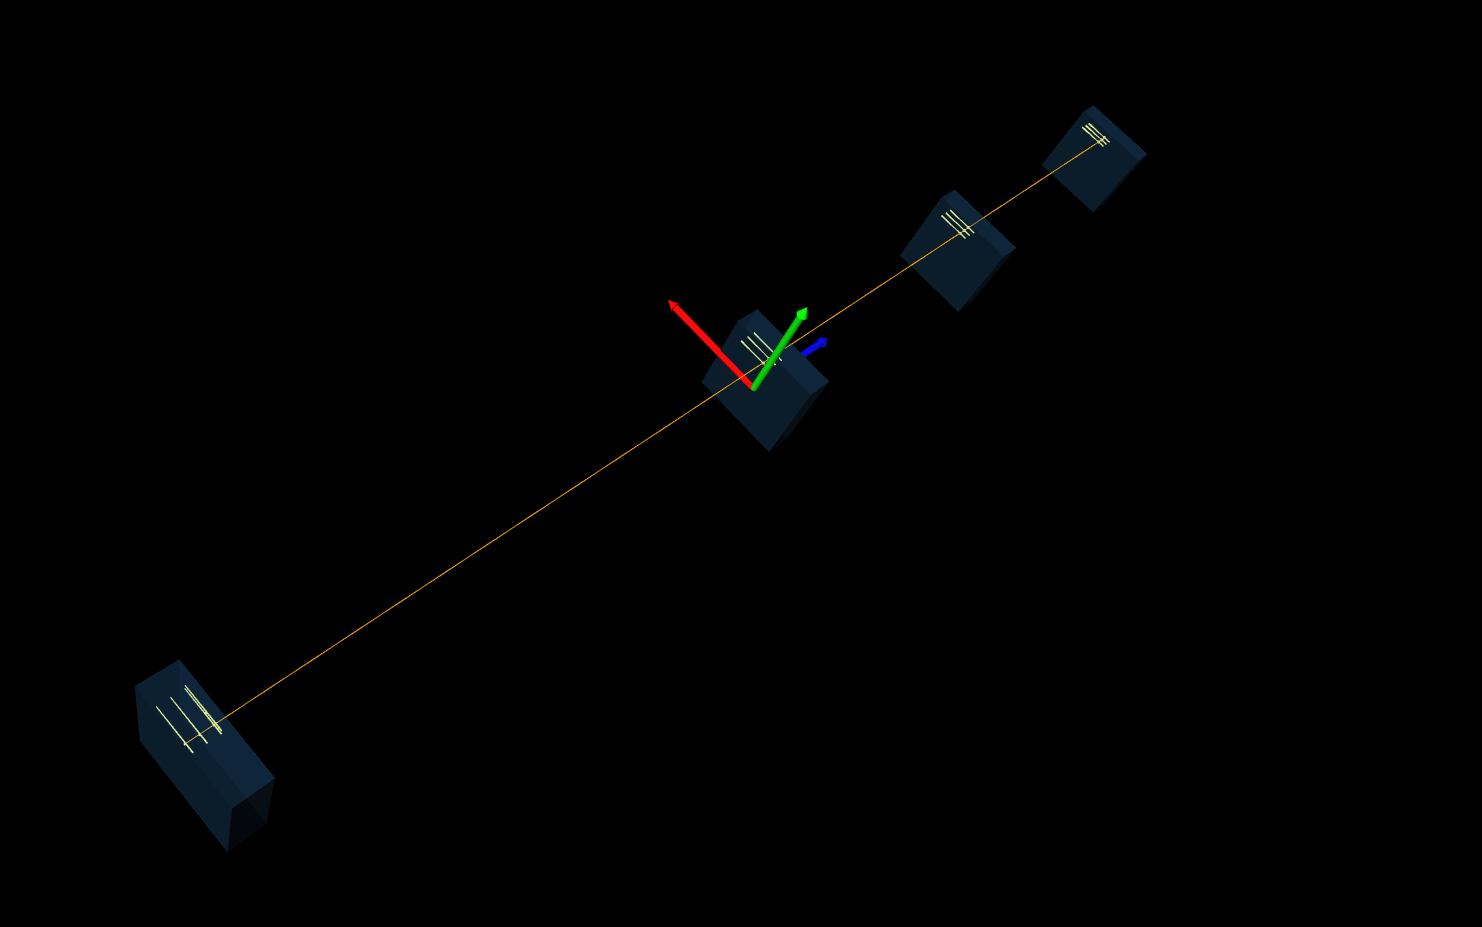
\includegraphics[width=0.7\textwidth]{assets/Event_Patched.png}};

            \draw[red, thick]
            ($(img.north west)!0.65!(img.north east) + (-0.5,-1)$)
            rectangle
            node (rect) {}
            ($(img.north west)!0.68!(img.north east) + (0.2,-2.3)$);

            \node[red, font=\footnotesize, anchor=north west, align=center] at ($(rect.south east)+(0.02,-0.01)$)
            {Regained two clusters?\\(St2, L2, Mod.3)};
        \end{tikzpicture}
        \caption{Event \#{2840829}, Run \#{022300} after disabling the error check mentioned above.}
    \end{figure}

    % \begin{itemize}
    %     \item Note that in this case the track is still reconstructed.
    %     \item Although it now has two missing clusters, which is not ideal.
    % \end{itemize}

\end{frame}

\begin{frame}
    \frametitle{Summary}

    \begin{itemize}
        \item Some issues was observed in the 2026 Tracker data.
              \begin{itemize}
                  \item Specifically in St2, L2, Mod.3 didn't seem to have any hits/clusters
                  \item This could probably be isolated to a specific chip
                  \item Studies still ongoing to better understand this.
              \end{itemize}
        \item The full extent of the impact on tracking is unclear
              \begin{itemize}
                  \item Probably not too huge
                  \item Could use some studies to quantify this.
              \end{itemize}
        \item We could use some better error handling in the reco. side
        \item Partly recovered by disabling some checks.
              \begin{itemize}
                  \item This is good which means we can recover at least some of the data if not all.
              \end{itemize}
    \end{itemize}



\end{frame}
